\section{Introduction}

Autonomous mobile robots (AMRs) in warehouses move through aisles they share with people. Their safety does not rest on the navigation software. An independent certified safety function monitors a protective field around the vehicle with a safety laser scanner and commands a stop when an object enters it \cite{iso3691-4,iec61496-3}. The field depends on the speed and direction of travel, and the stop latches until the field is clear and a restart condition holds. Production robots keep such certified scanners because software safety is hard to demonstrate to a safety body, and conservative fields can cause frequent stopping~\cite{liu2017}. Industrial studies of these fields measure their efficiency by fewer slowdowns and stops~\cite{muhammad2021}.

The navigation software above this layer is not certified, and it typically optimises navigation objectives without explicitly accounting for the geometry and the speed-dependent switching of the certified fields. Classical local planners represent obstacles by an inflation radius or a clearance cost \cite{coulter1992purepursuit,macenski2023rpp,fox1997dwa}. Such a planner treats the certified field as an unknown region of the world, so nothing in its design keeps the robot out of it. A planner can therefore be collision-free in its own terms and still trigger a stop at shelf corners, in narrow aisles and next to obstacles that are missing from its map. Protective stops are essential safety responses to detected intrusions. Some of them, however, arise from a mismatch between the nominal commands and the modeled field geometry, and not from an unavoidable collision situation: an oracle tracker with privileged knowledge can traverse every route of our scenario sets without breaching the lowest band's field (Section 5.2). Such stops are avoidable operational interruptions, and reducing them while the certified layer stays independent and active is the aim of this paper. Figure~\ref{fig:motivation} shows one such stop and the filtered alternative on a tuning scenario. Each trigger costs a restart delay and, in the worst case, a deadlock in which the restart condition never clears. On a certified vehicle the layer itself largely bounds collisions, so the operational cost that remains is the protective stop. We therefore take protective stops per 100 m of planned route as the primary metric, and report success, timeouts and mission time beside it, because a controller can lower its stop count by moving little.

\begin{figure}[t]
\centering
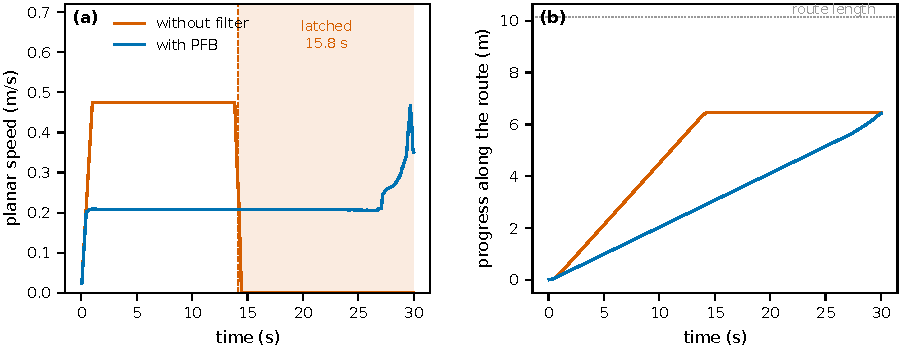
\includegraphics[width=\linewidth]{fig_motivation.pdf}
\caption{The operational cost of one protective stop, in an emulated run on the first narrow-aisle tuning scenario (planned route 10.1~m). A scan-blind route tracker, used only as an illustrative requested-command generator, drives the route twice with the certified layer beneath it. Without the filter it triggers one protective stop at 14~s (dashed line), and the latch (shaded) does not release within the 30~s window, because the declared recovery is not part of this emulation. With the PFB it triggers no stop but moves at a lower speed, and neither run reaches the goal within the window. (a) Planar speed. (b) Progress along the planned route.}
\label{fig:motivation}
\end{figure}

Control barrier functions (CBFs) constrain a command so that a safe set stays forward invariant \cite{ames2017cbfqp}. Used as a safety filter, a small quadratic program (QP) returns the admissible command closest to the one a controller requested. Filters of this kind are well established. Beam-wise discrete-time barrier constraints on LiDAR returns have been used with a constant safety margin~\cite{olayemi2026}. Filters of this kind can also stall a robot at undesired equilibria~\cite{mestres2026}. In the filters we reviewed, the safe set is a clearance chosen by the designer~\cite{olayemi2026}, and not the geometry and speed-regime switching of an external protective-field system. We do not claim a new barrier function, and the filter we use belongs to this family.

Among the works we reviewed, none protects a latching, speed-banded certified layer with a restart condition, and none evaluates a filter in that layer's own cost, protective stops, across controllers. This paper studies that case for classical local planners that do not account for the certified field, which we call field-blind. We evaluate three of them, pure pursuit, regulated pure pursuit and a holonomic dynamic window planner, and treat the dynamic window planner as the lead case, since it is the strongest of the three. We use the Protective-Field Barrier (PFB), a discrete-time barrier filter defined on the sectors of the laser scan, whose field mirrors the speed-banded protective field of the certified layer. The PFB sits between any controller and the layer. The filter modifies the nominal command to satisfy a one-step protective-field exclusion constraint under the assumed robot and sensing models: over one prediction horizon, no valid scan return may lie inside the modeled protective field of the speed regime the robot will be in. The filter solves one QP per speed regime for a holonomic base, brakes at the maximum rate when no regime is feasible, and is the identity when switched off. It is a candidate barrier: we do not show that it is a valid CBF, and we claim no safety guarantee beyond the emulated layer. The filter does not replace the certified layer, which remains independent and active.

The contributions are as follows.

\begin{itemize}
\item \emph{Methodological.} A protective-field-aware filtering formulation. The PFB places a barrier field that mirrors the speed-banded field of the certified layer between a controller and that layer, for a holonomic base with wheel-speed and acceleration limits, as an application of beam-wise discrete-time LiDAR barrier filters (Section 4).
\item \emph{Integration.} A controller-independent placement of the filter beneath three field-blind classical local planners, with the filter as the identity when switched off, so that a controller with and without it differs in one respect (Section 4).
\item \emph{Experimental.} A paired evaluation of protective stops, an explicit operational metric, beside success, timeouts and mission time, with an emulated certified layer beneath every controller. It establishes where the filter removes avoidable stops of field-blind planners and where it leaves routes incomplete when an obstacle is missing from the map, and it adds the sensitivity of the stops to the barrier gain (Sections 5 and 6). The results on the validation sets are exploratory, and the confirmatory comparison HF-c on the sealed test set covers regulated pure pursuit (Sections 5.6 and 6.2) \tbd{Section 6.4}
\end{itemize}

Section 2 reviews related work. Section 3 gives the preliminaries and the problem statement, Section 4 the filter and the controllers it sits beneath, Section 5 the experimental design, Section 6 the results, Section 7 the discussion, Section 8 the future work, and Section 9 concludes.

